\subsection{Experimental Results}
\label{sec:results}

We evaluated \jsynvg by synthesizing implementations
for 124 contracts%
\footnote{All of the benchmark contracts can be found at
\url{https://goo.gl/2p4sT9}.}
originated from a broad variety of contexts. Since we have been unable to find past work that contained benchmarks directly relevant to our approach, we propose a comprehensive collection of contracts that can be used by the research community for future advancements in reactive system synthesis for contracts that rely on infinite theories. Our benchmark collection is composed of the following three categories:
\begin{itemize}
\item 59 contracts correspond to various industrial projects, such as a Quad-Redundant Flight Control System, a Generic Patient Controlled Analgesia infusion pump, as well as a collection of contracts
for a Microwave model, written by graduate students as part of a software
engineering class;
\item 54 contracts were initially used for the verification of existing handwritten implementations~\cite{hagen2008scaling};
\item 11 models contain variations of the
Cinderella-Stepmother game, as well as examples that we created.
\end{itemize}
All of the synthesized implementations were verified against the original contracts using \jkind.

The goal of this experiment was to determine the performance and generality of the \jsynvg algorithm.  We compared against the existing \jsyn algorithm, and for the Cinderella model, we compared against~\cite{beyene2014constraint} (this was the only synthesis problem in the paper).  We examined the following aspects:
\begin{itemize}
    \item Time required to synthesize an implementation
    \item Size of generated implementations (in SLOC)
    \item Execution speed of generated C implementations derived from the synthesis procedure.
    \item Number of contracts that could be synthesized by each approach
\end{itemize}
\noindent Since \jkind already supports synthesis through \jsyn, we were able to directly
compare \jsynvg against \jsyn's $k$-inductive approach. We
ran the experiments using a computer with Intel Core i3-4010U 1.70GHz CPU and
16GB RAM.

% \begin{table}[!t]
% \centering
% \hspace{-25pt}
% \begin{minipage}{0.4\textwidth}
% %\begin{table}[!t]
% \centering
% \caption{Benchmark Statistics}
% \label{tbl:stats}
% \resizebox{\textwidth}{!}{%
% \begin{tabular}{@{}lll@{}}
% \toprule
%  & \jsyn & \jsynvg \\ \midrule
% Problems solved & 113 & \textbf{124} \\
% Performance (avg - seconds) & 5.72 & \textbf{2.78} \\
% Performance (max - seconds) & 352.1 & \textbf{167.55} \\
% Implementation Size (avg - Lines of Code) & 72.88 & \textbf{70.66} \\
% Implementation Size (max - Lines of Code) & 2322 & \textbf{2142} \\
% Implementation Performance (avg - ms) & 57.84 & \textbf{56.32} \\
% Implementation Performance (max - ms) & 485.88 & \textbf{459.95} \\
% \bottomrule
% \end{tabular}
% }
% %\end{table}
% \end{minipage}
% \begin{minipage}{0.55\textwidth}
% %\begin{table*}[!t]
% \centering
% \caption{Cinderella-Stepmother results}
% \label{tbl:cindtbl}
% \resizebox{1.1\textwidth}{!}{%
% \begin{tabular}{|c|c|c|c|c|c|}
% \hline
% \multirow{2}{*}{Game} & \multicolumn{3}{c|}{\jsynvg} & \multicolumn{2}{c|}{\textsc{ConSynth}~\cite{beyene2014constraint}} \\ \cline{2-6}
%  & \begin{tabular}[c]{@{}c@{}}Impl. Size\\ (LoC)\end{tabular} & \begin{tabular}[c]{@{}c@{}}Impl. Performance\\ (ms)\end{tabular} & Time & \begin{tabular}[c]{@{}c@{}}Time\\ (Z3)\end{tabular} & \begin{tabular}[c]{@{}c@{}}Time\\ (Barcelogic)\end{tabular} \\ \hline
% Cind (C = 3) & 204 & 128.09 & 4.5s & \multirow{2}{*}{3.2s} & \multirow{2}{*}{1.2s} \\ \cline{1-4}
% Cind2 (C = 3) & 2081 & 160.87 & 28.7s &  &  \\ \hline
% Cind (C = 2) & 202 & 133.04 & 4.7s & \multirow{2}{*}{1m52s} & \multirow{2}{*}{1m52s} \\ \cline{1-4}
% Cind2 (C = 2) & 1873 & 182.19 & 27.2s &  &  \\ \hline
% \end{tabular}
% }
%\end{table*}
A listing of the statistics that we tracked while running experiments is
presented in Table~\ref{tbl:stats}.
Fig.~\ref{fg:performance} shows the time allocated by \jsyn and \jsynvg to solve each problem, with \jsynvg
outperforming \jsyn for the vast majority of the benchmark suite, often times by a margin greater than
50\%. Fig.~\ref{fg:size} on the other hand, depicts small differences in the
overall size between the synthesized implementations. While it would be
reasonable to conclude that there are no noticable improvements, the big picture is different. The key factor that is not apparent from this figure, is the length of the $k$-inductive proof. For the majority of the benchmarks in the suite, \jsyn proves their realizability by constructing proofs of length $k=0$, which essentially means that the entire space of states is an inductive invariant. For these cases, both algorithms generate a single Skolem function. In the general case though, the size of \jsyn solutions is directly
dependent on $k$, since each implementation is composed of $k$ Skolem
functions ($k-1$ to initialize the system, and one last for the inductive step),
where the equivalent solution from \jsynvg is always just one.
Fig.~\ref{fg:size} hints towards this intuition, through several spikes
in \jsyn implementation size. Despite this, we also noticed cases where \jsyn
implementations are shorter. This provides us with another interesting
observation regarding the formulation of the problem for $k=0$ proofs. In
these cases, \jsyn proves the existence of viable states, starting from a set
of \textit{pre-initial} states, where the contract does not need to hold. This
has direct implications to the way that the $\forall\exists$-formulas are
constructed in \jsyn's underlying machinery, where the assumptions are ``baked''
into the transition relation, affecting thus the performance of \aeval.

\begin{table}[!t]
\centering
\hspace{-25pt}
\begin{minipage}{0.45\textwidth}
%\begin{table}[!t]
\centering
\caption{Benchmark Statistics}
\label{tbl:stats}
\resizebox{\textwidth}{!}{%
\begin{tabular}{|l|c|c|}
%\toprule
\hline
 & \jsyn & \jsynvg \\ \hline % \midrule
Problems solved & 113 & \textbf{124} \\ \hline
Performance (avg - seconds) & 5.72 & \textbf{2.78} \\ \hline
Performance (max - seconds) & 352.1 & \textbf{167.55} \\ \hline
Implementation Size (avg - Lines of Code) & 72.88 & \textbf{70.66} \\ \hline
Implementation Size (max - Lines of Code) & 2322 & \textbf{2142} \\ \hline
Implementation Performance (avg - ms) & 57.84 & \textbf{56.32} \\ \hline
Implementation Performance (max - ms) & 485.88 & \textbf{459.95} \\ \hline
%\bottomrule
\end{tabular}
}
%\end{table}
\end{minipage}
\begin{minipage}{0.48\textwidth}
%\begin{table*}[!t]
\centering
\vspace{-.82em}
\caption{Cinderella-Stepmother results}
\label{tbl:cindtbl}
\resizebox{1.1\textwidth}{!}{%
\begin{tabular}{|c|c|c|c|c|c|}
\hline
\multirow{2}{*}{Game} & \multicolumn{3}{c|}{\jsynvg} & \multicolumn{2}{c|}{\textsc{ConSynth}~\cite{beyene2014constraint}} \\ \cline{2-6}
 & \begin{tabular}[c]{@{}c@{}}Impl. Size\\ (LoC)\end{tabular} & \begin{tabular}[c]{@{}c@{}}Impl. Performance\\ (ms)\end{tabular} & Time & \begin{tabular}[c]{@{}c@{}}Time\\ (Z3)\end{tabular} & \begin{tabular}[c]{@{}c@{}}Time\\ (Barcelogic)\end{tabular} \\ \hline
Cind (C = 3) & 204 & 128.09 & 4.5s & \multirow{2}{*}{3.2s} & \multirow{2}{*}{1.2s} \\ \cline{1-4}
Cind2 (C = 3) & 2081 & 160.87 & 28.7s &  &  \\ \hline
Cind (C = 2) & 202 & 133.04 & 4.7s & \multirow{2}{*}{1m52s} & \multirow{2}{*}{1m52s} \\ \cline{1-4}
Cind2 (C = 2) & 1873 & 182.19 & 27.2s &  &  \\ \hline
\end{tabular}
}
\end{minipage}
\end{table}
One last statistic that we tracked was the performance of the synthesized C
implementations in terms of execution time, which can be seen in Fig.~\ref{fg:implperformance}. The performance was computed as the mean of 1000000 iterations of executing each implementation using rando input values.
 \iffalse
  For this purpose, we translated the
 generated witnesses from \jsyn and \jsynvg solutions using
 \smtlibtoc under the same set of options.
 \fi
 According to the figure as well as Table~\ref{tbl:stats}, the differences are minuscule on average.
\iffalse
while \jsyn implementations are faster, the difference is minuscule on average.
This small difference may occur due to the fact that \jsyn creates separate skolem functions for the initial evaluation
(when \%init is true)

and subsequent evaluations, whereas currently \jsynvg uses a single function for both cases, and as such requires the evaluation of richer expressions prior to choosing a proper reaction.
\fi

% The deciding factor in this context is the
% difference in complexity of the Model-Based Projections that get generated by
% \aeval using \jsyn and \jsynvg, with the latter versions containing richer
% expressions, mainly due to the refinement process.

\begin{figure}[!t]
\centering
\subfloat[Performance of synthesizers]{
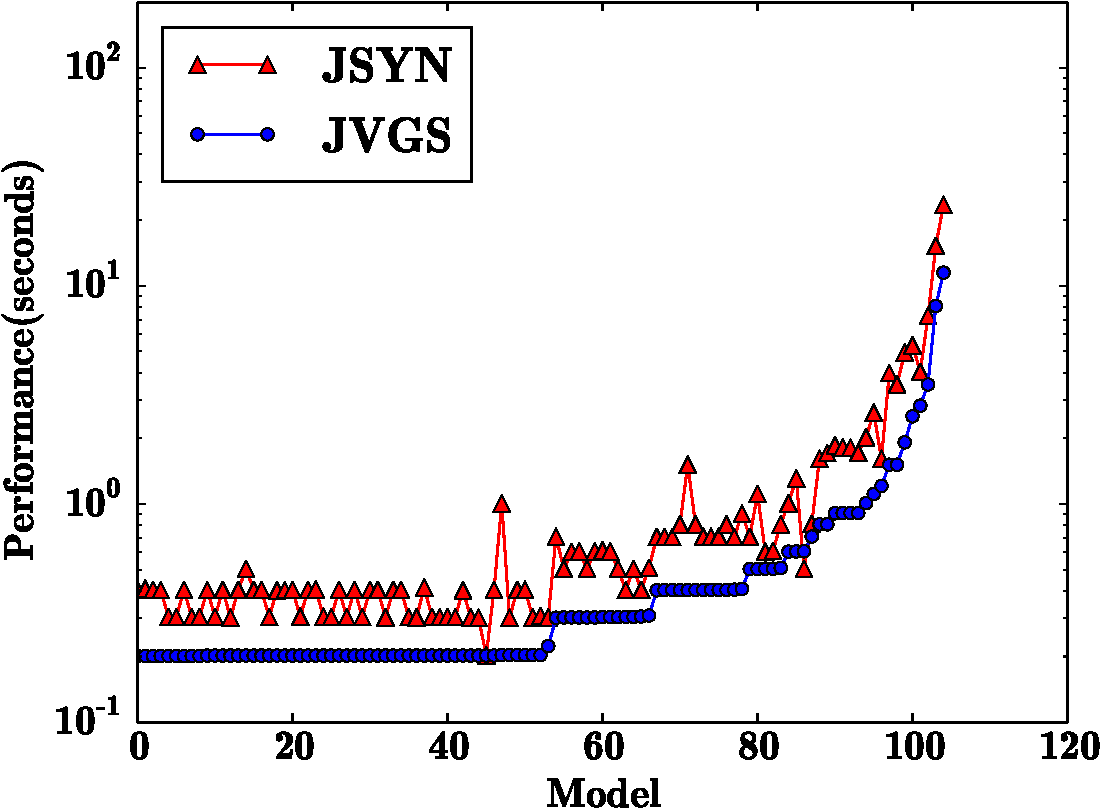
\includegraphics[width=2in]{overhead-crop}
\label{fg:performance}}
%\hspace{+6.5em}
\quad
\subfloat[Size of implementations]{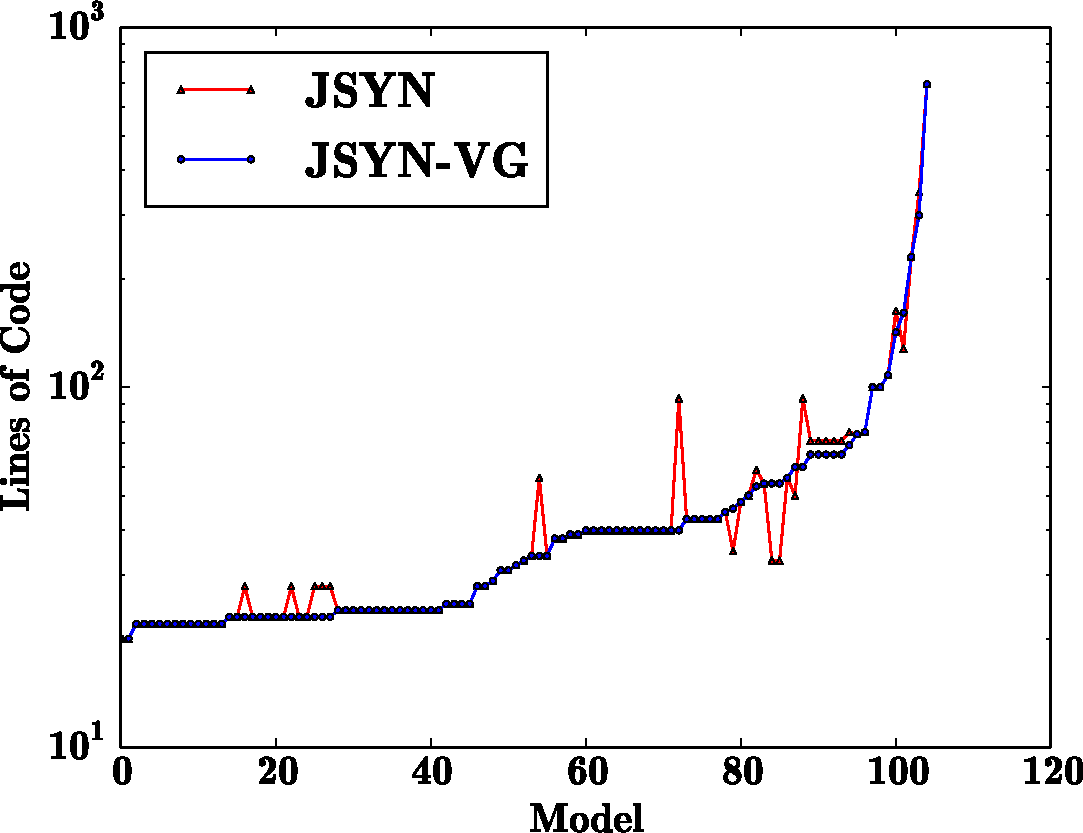
\includegraphics[width=2in]{loc-crop}
\label{fg:size}}
\quad
\subfloat[Performance of implementations]{
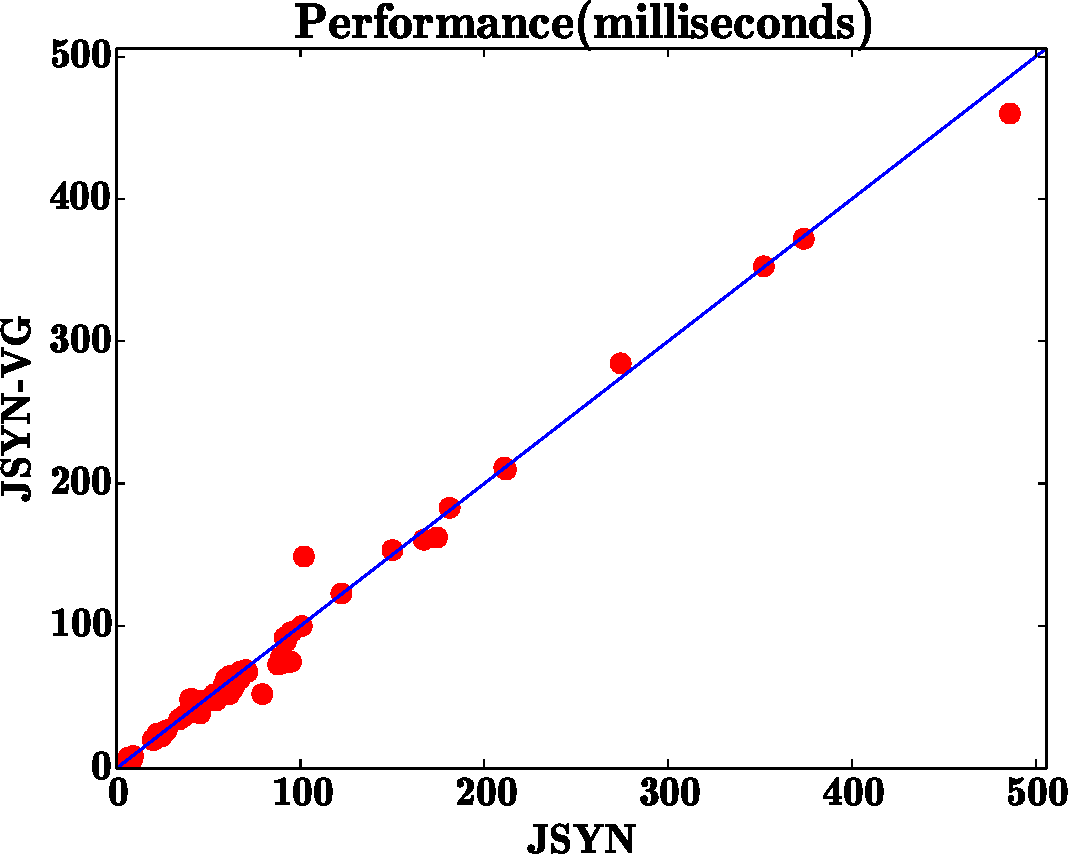
\includegraphics[width=2in]{performance-crop}
\label{fg:implperformance}}
\caption{Experimental results}
\vspace{-5pt}
\label{fg:results}
\end{figure}


Fig.~\ref{fg:results} does not cover the entirety of the
benchmark suite. From the original 124 problems, eleven of them cannot be
solved by \jsyn's $k$-inductive approach.
%\grigory{ideally, a summary of these observations should be pulled all the way towards the intro. Even more, It should probably be the main motivation of the entire work.}
Four of these files are variations of
the Cinderella-Stepmother game using different representations of the game, as well as two different values
for the bucket capacity (2 and 3). Using the variation in Fig.~\ref{fg:cind} as an input to \jsyn, we receive an ``unrealizable'' answer, with the counterexample shown
in Fig.~\ref{fg:cex}. Reading through the feedback provided by \jsyn, it is
apparent that the underlying SMT solver is incapable of choosing the correct
buckets to empty, leading eventually to a state where an overflow occurs for the
third bucket. As we already discussed though, a winning strategy exists for the
Cinderella game, as long as the bucket capacity \texttt{C} is between 1.5 and 3. This
provides an excellent demonstration of the inherent weakness of \jsyn
for determining unrealizability. \jsynvg's validity-guided approach,
is able to prove the realizability for these contracts, as
well as synthesize an implementation for each.

\begin{figure}[!t]
\centering
 \begin{Verbatim}[fontsize=\scriptsize]
	 ++++++++++++++++++++++++++++++++++++++++++++++++++++++++++
	      UNREALIZABLE || K = 6 || Time = 2.017s
	                 Step
	      variable      0    1      2      3      4      5
	      INPUTS
	      i1            0    0      0 0.416* 0.944* 0.666*
	      i2            1    0 0.083* 0.083*      0 0.055*
	      i3            0    1 0.305*    0.5 0.027* 0.194*
	      i4            0    0 0.611*      0      0 0.027*
	      i5            0    0      0      0 0.027* 0.055*
	
	      OUTPUTS
	      e             1    3      1      5      4      5
	
	      NODE OUTPUTS
	      guarantee   true true   true   true   true  false
	
	      NODE LOCALS
	      b1            0    0      0 0.416* 1.361* 0.666*
	      b2            0    0 0.083* 0.166* 0.166* 0.222*
	      b3            0    1 1.305* 1.805* 1.833* 2.027*
	      b4            0    0 0.611* 0.611*      0 0.027*
	      b5            0    0      0      0 0.027* 0.055*
	
	      * display value has been truncated
	 ++++++++++++++++++++++++++++++++++++++++++++++++++++++++++
 \end{Verbatim}
\vspace{-1.5em}
\caption{Spurious counterexample for Cinderella-Stepmother example using \jsyn}
\label{fg:cex}
\end{figure}

% \begin{table*}[!t]
% \centering
% \caption{Cinderella-Stepmother results}
% \label{tbl:cindtbl}
% \resizebox{0.7\textwidth}{!}{%
% \begin{tabular}{|c|c|c|c|c|c|}
% \hline
% \multirow{2}{*}{Game} & \multicolumn{3}{c|}{\jsynvg} & \multicolumn{2}{c|}{\textsc{ConSynth}~\cite{beyene2014constraint}} \\ \cline{2-6}
%  & \begin{tabular}[c]{@{}c@{}}Impl. Size\\ (LoC)\end{tabular} & \begin{tabular}[c]{@{}c@{}}Impl. Performance\\ (ms)\end{tabular} & Time & \begin{tabular}[c]{@{}c@{}}Time\\ (Z3)\end{tabular} & \begin{tabular}[c]{@{}c@{}}Time\\ (Barcelogic)\end{tabular} \\ \hline
% Cind (C = 3) & 204 & 128.09 & 4.5s & \multirow{2}{*}{3.2s} & \multirow{2}{*}{1.2s} \\ \cline{1-4}
% Cind2 (C = 3) & 2081 & 160.87 & 28.7s &  &  \\ \hline
% Cind (C = 2) & 202 & 133.04 & 4.7s & \multirow{2}{*}{1m52s} & \multirow{2}{*}{1m52s} \\ \cline{1-4}
% Cind2 (C = 2) & 1873 & 182.19 & 27.2s &  &  \\ \hline
% \end{tabular}}
% \end{table*}
% \begin{table*}[!t]
% \centering
% \caption{Cinderella-Stepmother results}
% \label{tbl:cindtbl}
% \begin{tabular}{|c|c|c|c|c|c|}
% \hline
%  & \multicolumn{3}{c|}{\jsynvg} & \multicolumn{2}{c|}{\textsc{ConSynth}~\cite{beyene2014constraint}} \\ \hline
%  & Implementation Size (LoC) & Implementation Performance (ms) & Time & Time (Z3) & Time (Barcelogic) \\ \hline
% Cinderella (C = 3) & 92 & 262.84 & 35s & \multirow{2}{*}{3.2s} & \multirow{2}{*}{1.2s} \\ \cline{1-4}
% Cinderella2 (C = 3) & 222 & 309.24 & 2m9s &  &  \\ \hline
% Cinderella (C = 2) & 102 & 196.57 & 24s & \multirow{2}{*}{1m52s} & \multirow{2}{*}{1m52s} \\ \cline{1-4}
% Cinderella2 (C = 2) & 272 & 230.16 & 2m9s &  &  \\ \hline
% \end{tabular}
% \end{table*}

Table~\ref{tbl:cindtbl} shows how \jsynvg performed on the four contracts describing the Cinderella-Stepmother game. We used two different interpretations for the game, and exercised both for the cases where the bucket capacity  \texttt{C} is equal to 2 and 3. Regarding the synthesized implementations, their size is analogous to the complexity of the program (Cinderella2 contains more local variables and a helper function to empty buckets). Despite this, the implementation performance remains the same across all implementations. Finally for reference, the table contains the results from the template-based approach followed in \textsc{Consynth}~\cite{beyene2014constraint}. From the results, it is apparent that providing templates yields better performance for the case of $C = 3$, but our approach overperforms \textsc{Consynth} when it comes to solving the harder case of $C = 2$. As a final remark, the original paper for \textsc{Consynth} also explores the synthesis of winning strategies for Stepmother using the liveness property that a bucket will eventually overflow. While \jkind does not natively support liveness properties, we successfully synthesized an implementation for Stepmother using a bounded notion of liveness with counters. We leave an evaluation of this category of specifications for future work.

Overall, \jsynvg's validity-guided approach provides significant advantages
over the $k$-inductive technique followed in \jsyn, and effectively expands
\jkind's solving capabilities regarding specification realizability. On top of that, it provides an efficient ``hands-off'' approach that is capable of solving complex games.
The most significant contribution, however, is the applicability of this approach, as it is not tied to a specific environment since it can be extended to support more
theories, as well as categories of specification. 